\documentclass{article}

\usepackage{microtype}
\usepackage{graphicx}
\usepackage{subfigure}
\usepackage{booktabs} % for professional tables


\usepackage{hyperref}
\usepackage{array}

% Attempt to make hyperref and algorithmic work together better:
\newcommand{\theHalgorithm}{\arabic{algorithm}}


\usepackage[accepted]{icml2021}

% The \icmltitle you define below is probably too long as a header.
% Therefore, a short form for the running title is supplied here:
\icmltitlerunning{Image Animation with Keypoint Mask}

\begin{document}

\twocolumn[
\icmltitle{Image Animation with Keypoint Mask}

\icmlsetsymbol{equal}{*}

\begin{icmlauthorlist}
\icmlauthor{Or Toledano}{tlv}
\icmlauthor{Yanir Marmor}{tlv}
\icmlauthor{Dov Gertz}{tlv}

\end{icmlauthorlist}

\icmlaffiliation{tlv}{Tel Aviv University}

\icmlcorrespondingauthor{Or Toledano}{ortoledano@protonmail.com}
\icmlcorrespondingauthor{Yanir Marmor}{yanirmr@gmail.com}
\icmlcorrespondingauthor{Dov Gertz}{TODO}


\icmlkeywords{Machine Learning, ICML}

\vskip 0.3in
]
\printAffiliationsAndNotice{}  % leave blank if no need to mention equal contribution
%\printAffiliationsAndNotice{\icmlEqualContribution} % otherwise use the standard text.

\begin{abstract}
Image animation is the task of synthesizing future video frames of a single
source image according to the motion from a driving video.
This task is challenging due to the complexity of motion representation
and the unknown relations between the driving video and the source image.
Despite this difficulty, this problem attracted great interests from
researches at the recent years, with gradual improvements. The
problem can be thought as decoupling of motion and appearance, which is
often solved by extracting the motion from keypoint movement. In this work,
we extract the structure by a keypoint heatmap, without an explicit
motion representation. Then, the structures from the image and the video
are extracted to warp the image according to the video, by a deep
generator. Our approach outperforms the state of the art in popular
reconstruction benchmarks, and an improvement can be easily observed in
animating videos.
\cite{siarohin2020order} % @Or - why this citation is here?
\end{abstract}

\section{Introduction}

% add some words about good and evil use in this technique

\cite{10.1145/3425780} in their survey about Creation and Detection of Deepfakes split this area into four categories of tasks:
reenactment, replacement, editing,
and synthesis.


our project focus involved at the "replacement" category.

TODO: didn't you mean synthesis?

The main challenges we need to deal with, as they defined in that survey are: paired training, identity leakage, occlusions and temporal coherence,



Our paper focuses on the motion transfer problem: given a source image $S$
and a driving video $D$, the goal is to syntesize a video with the identity
of $S$, and the motion from $D$.
Some notable works \cite{siarohin2020order}, \cite{wiles2018x2face},
\cite{siarohin2019animating}.

Our method does not rely on GANs - see Section~\ref{method}.

our contribution it twofold: first, ignore the motion prior and better accuracy results, and second compact representation with better performance.

\medskip

\textbf{Related Work:} Our work doesn't rely directly on a strong motion prior,
but uses a structure mask which was extracted from a keypoint detector
of a motion based model, such as \cite{siarohin2020order}. The concept of using drawn keypoints as
a geometry represantation (structural mask) was already used in the context
of image-to-image translation, in works such as TransGaGa \cite{wu2019transgaga}.
The concept of using a structural mask in the context of image animation is
demonstrated in \cite{shalev2020image}. However, the current work differs
by basing the mask off a motion related module, which saves us the hassle
of perturbing the input hoping to achieve an identy-less mask. That way, we
can base more of the motion representation on the deep network, reduce our
prior, and leave some space for our network to achieve better results.


\subsection{Keypoints}
In contrast to pixel-based approaches that were prevalent until a few years ago.
Recently, keypoint-based approaches have been perceived as having the
potential to achieve high performance in the field of video prediction.
\cite{kim2019unsupervised}, \cite{balakrishnan2018synthesizing}
\cite{ma2017pose}  \cite{reed2017parallel} \cite{chan2019everybody}
\cite{villegas2017learning}
\cite{cai2018deep}
\cite{wang2018every}
\cite{reed2015deep}

 However, these works require frame-by-frame keypoints labeling, which limits the applicability of the methods. There are several of solutions for this problem. Basically, we need to use a pre-trained keypoints detector for our model. (relevant cites for that: \cite{siarohin2019animating} \cite{thewlis2017unsupervised} \cite{zhang2018unsupervised} \cite{jakab2018unsupervised} \cite{newell2016stacked})
\section{Methodology}
\label{method}

\begin{figure}[ht]
\vskip 0.2in
\begin{center}
\centerline{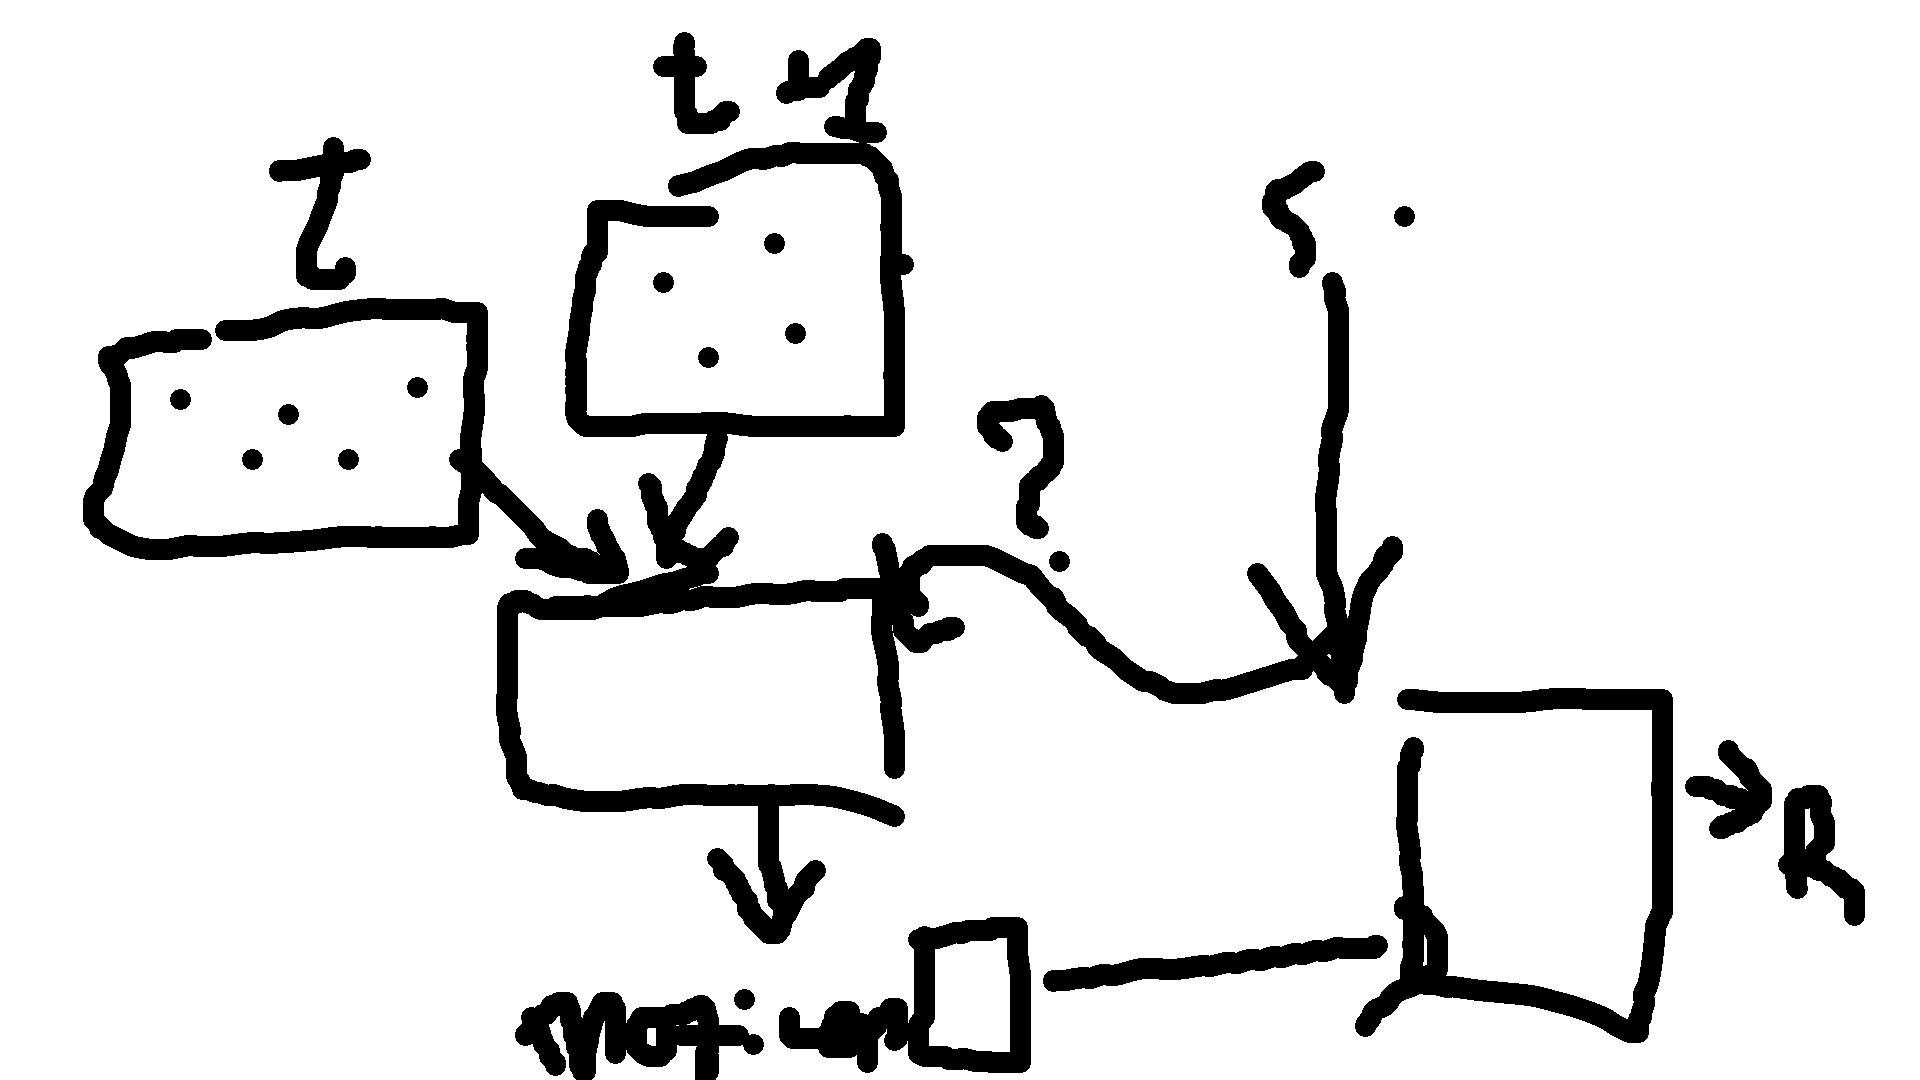
\includegraphics[width=\columnwidth]{second_meeting_pres}}
\caption{
Architecture
}
\label{arch}
\end{center}
\vskip -0.2in
\end{figure}


\begin{figure}[ht]
\vskip 0.2in
\begin{center}
\centerline{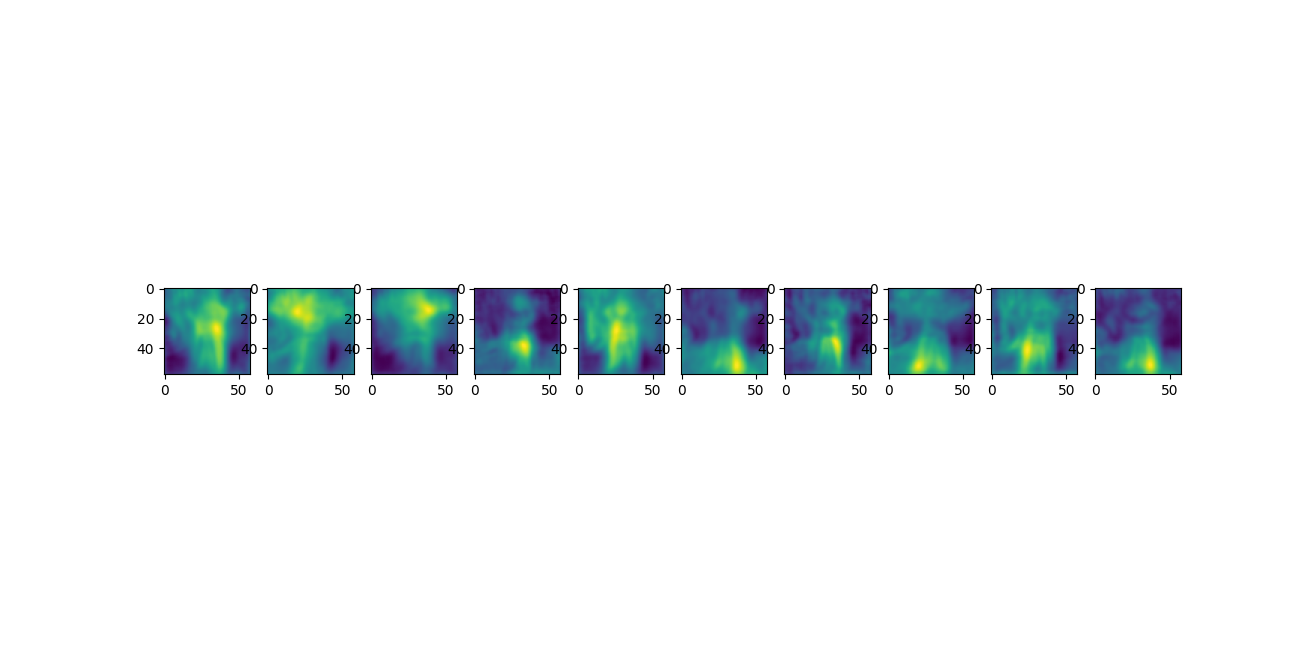
\includegraphics[width=\columnwidth]{mask_10kp}}
\caption{
$K$ channels of the keypoint detector network used in
\cite{siarohin2020order}, before the softmax activation. Our main motion
prior in this project.
}
\label{mask-10kp}
\end{center}
\vskip -0.2in
\end{figure}


\begin{figure}[ht]
\vskip 0.2in
\begin{center}
\centerline{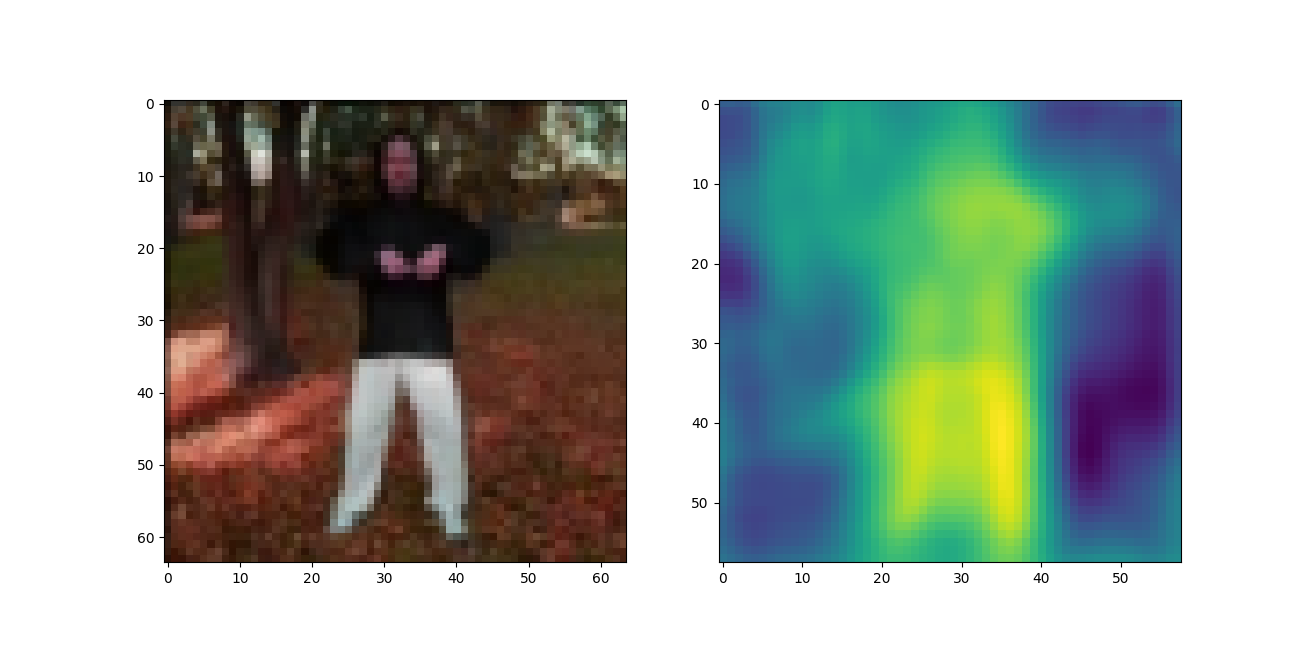
\includegraphics[width=\columnwidth]{mask_sum}}
\caption{
The sum of the $K$ channels which is fed as a structural mask into the
generator.
}
\label{mask-sum}
\end{center}
\vskip -0.2in
\end{figure}


\subsection{Losses}
Perceptual Vgg19 \cite{simonyan2015deep}
\subsection{Version for relative motion transfer}
We purposes an additional "circles" only mask
which can be used in the context
of relative motion transfer during animation, as in
\cite{siarohin2020order}, which isn't possible with a mask.
The masks catches the geometry representation \cite{wu2019transgaga} of the
image, and by forcing it to be described as keypoints with a center, we can
use the relative coordinates for the animation. However, this module didn't
perform as well as our heatmap mask module (~\label{table:results}).
Relative motion transfer isn't always the wanted outcome, but this work
indicates that a keypoint-only-prior based module is feasible for the task.


\begin{figure}[ht]
\vskip 0.2in
\begin{center}
\centerline{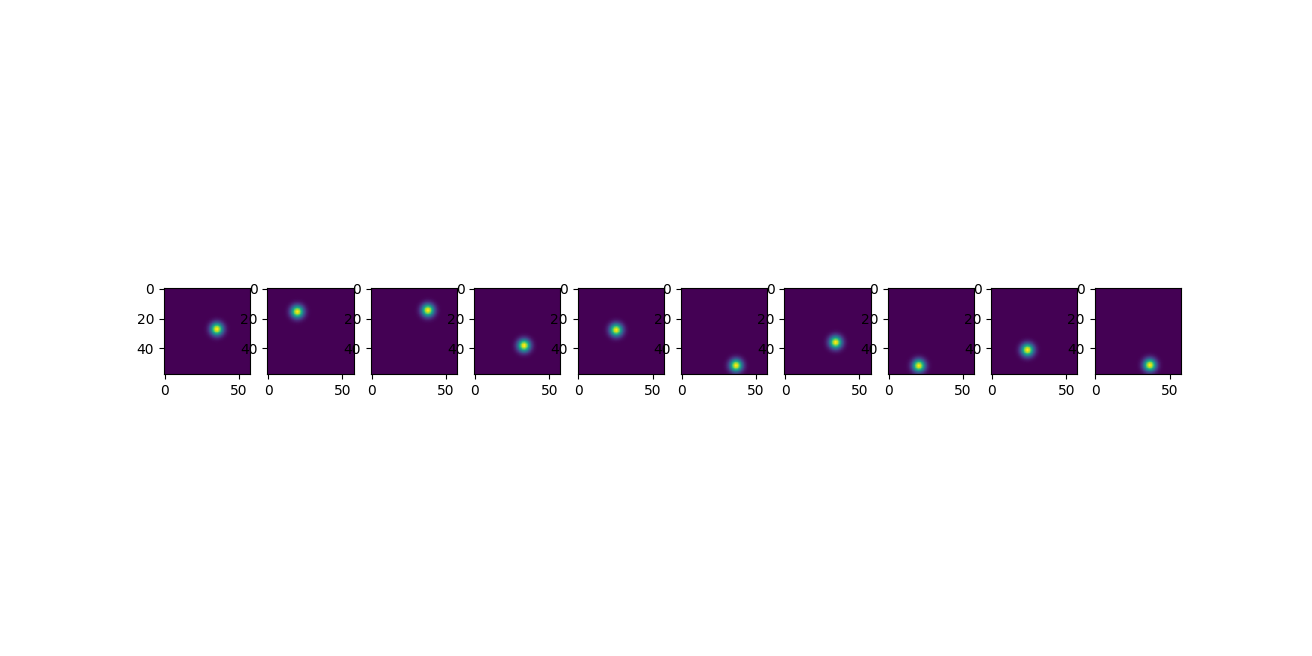
\includegraphics[width=\columnwidth]{softmax_10kp}}
\caption{
$K$ channels of the keypoint detector network used in
\cite{siarohin2020order}, after the softmax activation and Gaussian fit.
}
\label{softmax-10kp}
\end{center}
\vskip -0.2in
\end{figure}


\begin{figure}[ht]
\vskip 0.2in
\begin{center}
\centerline{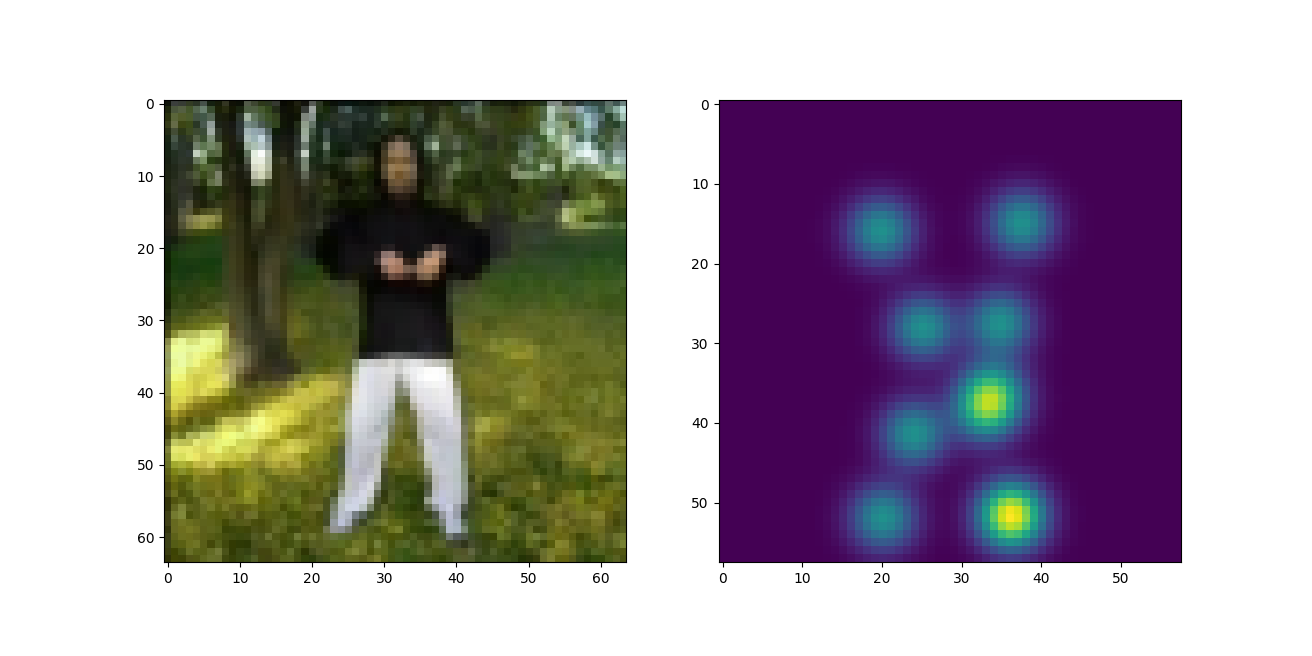
\includegraphics[width=\columnwidth]{softmax_sumkp}}
\caption{
The sum of the $K$ channels which is fed as a structural mask into the
generator.
}
\label{softmax-sum}
\end{center}
\vskip -0.2in
\end{figure}

\section{Experiments}
\subsection{Datasets}
The training and evaluation were done using Tai-Chi-HD dataset which containing short videos of people doing tai-chi exercises. Following \cite{siarohin2020order}, 3,141 tai-chi videos were downloaded from YouTube. The videos were cropped and resized to a resolution of $256^2$, while preserving the aspect ratio. There are 3,016 training videos and 125 test videos.

\begin{table}[t]
\caption{Images comparison}
\label{table:images}
\vskip 0.15in
\begin{center}
\begin{small}
\begin{sc}
\begin{tabular}{m{1.0cm}m{1.0cm}m{1.0cm}m{1.0cm}m{1.0cm}m{1.0cm}}
\toprule
Source image & Driving\\
\toprule
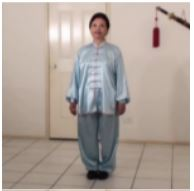
\includegraphics[width=1cm, height=1cm]{images/source.JPG} &
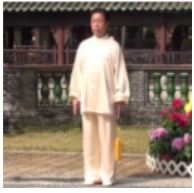
\includegraphics[width=1cm, height=1cm]{images/driving1.JPG} &
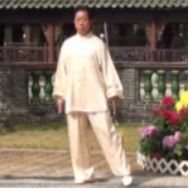
\includegraphics[width=1cm, height=1cm]{images/driving2.JPG} &
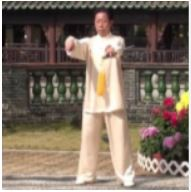
\includegraphics[width=1cm, height=1cm]{images/driving3.JPG} &
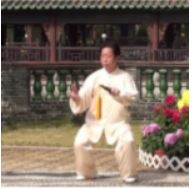
\includegraphics[width=1cm, height=1cm]{images/driving4.JPG} &
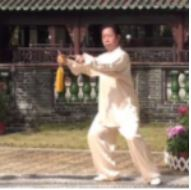
\includegraphics[width=1cm, height=1cm]{images/driving5.JPG} \\
\midrule
X2Face & 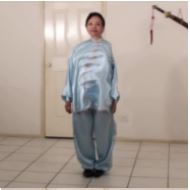
\includegraphics[width=1cm, height=1cm]{images/1_X2Face_1.JPG} &
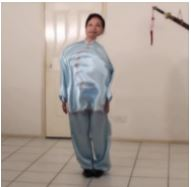
\includegraphics[width=1cm, height=1cm]{images/1_X2Face_2.JPG} &
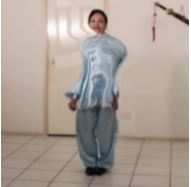
\includegraphics[width=1cm, height=1cm]{images/1_X2Face_3.JPG} &
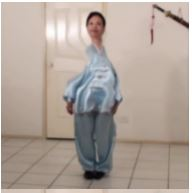
\includegraphics[width=1cm, height=1cm]{images/1_X2Face_4.JPG} &
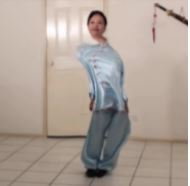
\includegraphics[width=1cm, height=1cm]{images/1_X2Face_5.JPG} \\
Monkey-Net & 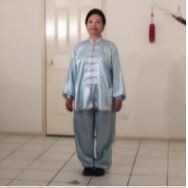
\includegraphics[width=1cm, height=1cm]{images/2_Monkey-Net_1.JPG} &
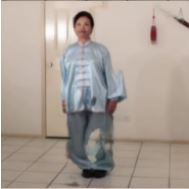
\includegraphics[width=1cm, height=1cm]{images/2_Monkey-Net_2.JPG} &
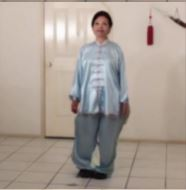
\includegraphics[width=1cm, height=1cm]{images/2_Monkey-Net_3.JPG} &
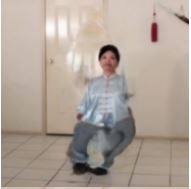
\includegraphics[width=1cm, height=1cm]{images/2_Monkey-Net_4.JPG} &
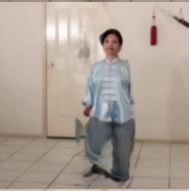
\includegraphics[width=1cm, height=1cm]{images/2_Monkey-Net_5.JPG} \\
FOMM & 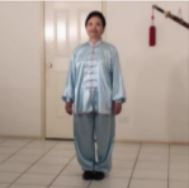
\includegraphics[width=1cm, height=1cm]{images/3_FOMM_1.JPG} &
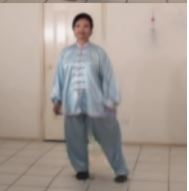
\includegraphics[width=1cm, height=1cm]{images/3_FOMM_2.JPG} &
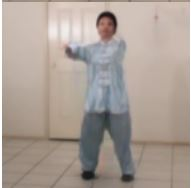
\includegraphics[width=1cm, height=1cm]{images/3_FOMM_3.JPG} &
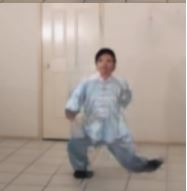
\includegraphics[width=1cm, height=1cm]{images/3_FOMM_4.JPG} &
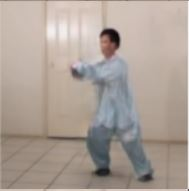
\includegraphics[width=1cm, height=1cm]{images/3_FOMM_5.JPG} \\
Perturbed Mask & 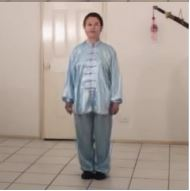
\includegraphics[width=1cm, height=1cm]{images/4_YOAV_1.JPG} &
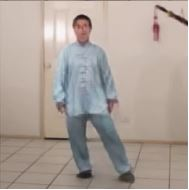
\includegraphics[width=1cm, height=1cm]{images/4_YOAV_2.JPG} &
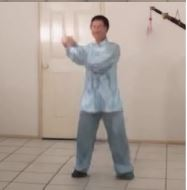
\includegraphics[width=1cm, height=1cm]{images/4_YOAV_3.JPG} &
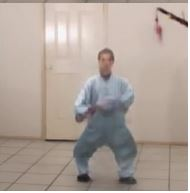
\includegraphics[width=1cm, height=1cm]{images/4_YOAV_4.JPG} &
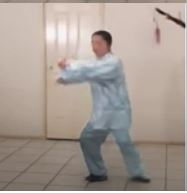
\includegraphics[width=1cm, height=1cm]{images/4_YOAV_5.JPG} \\
Ours & 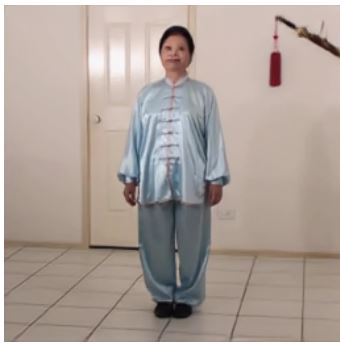
\includegraphics[width=1cm, height=1cm]{images/5_OURS_1.JPG} &
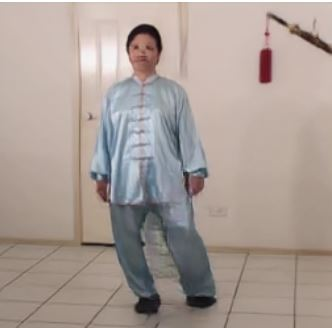
\includegraphics[width=1cm, height=1cm]{images/5_OURS_2.JPG} &
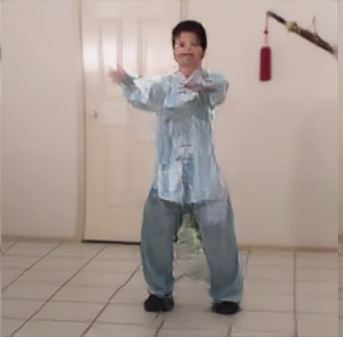
\includegraphics[width=1cm, height=1cm]{images/5_OURS_3.JPG} &
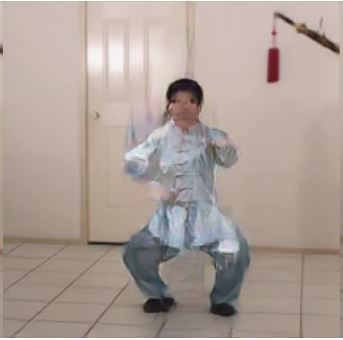
\includegraphics[width=1cm, height=1cm]{images/5_OURS_4.JPG} &
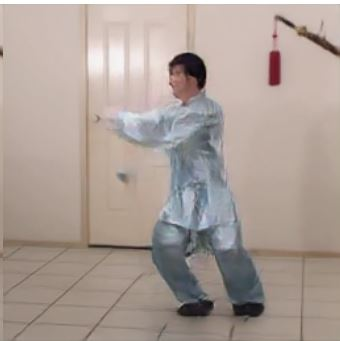
\includegraphics[width=1cm, height=1cm]{images/5_OURS_5.JPG} \\
\bottomrule
\end{tabular}
\end{sc}
\end{small}
\end{center}
\vskip -0.1in
\end{table}




\subsection{Comparison with Previous Works}
In order to compere our work to previous works(Table~\ref{table:results}) we used metrics previously used in similar papers. Average Key-points Distance \cite{cao2017realtime} (AKD) measures the average key-points distance between the generated video and the source video. Average Euclidean Distance \cite{zheng2019joint}  (AED) measures the average euclidean distance
 between the representations of the ground-truth and generated videos in some embedding space. In addition, we added the L1 distance as well. The AED and AKD metrics were calculated using the following github: https://github.com/AliaksandrSiarohin/pose-evaluation.


% Note use of \abovespace and \belowspace to get reasonable spacing
% above and below tabular lines.

\begin{table}[t]
\caption{Accuracy Metrics}
\label{table:results}
\vskip 0.15in
\begin{center}
\begin{small}
\begin{sc}
\begin{tabular}{lcccr}
\toprule
Method & AKD & AED & L1 \\
\midrule
Monkey-Net    & 10.798 & 0.228 & 0.077 \\
FOMM    & 6.872 & 0.167 & 0.063 \\
Perturbed Mask & 4.239 & 0.147 & 0.047 \\
Ours softmax & 14.760& 0.245 & 0.077 \\
Ours & 5.551 & 0.141 &  0.045\\
\midrule
Improvement (FOMM)    & 19.2\% & 15.5\% & 28.5\% \\
\bottomrule
\end{tabular}
\end{sc}
\end{small}
\end{center}
\vskip -0.1in
\end{table}
\section{Future work}
Test more datasets
Remove the explicit sum of channels, maybe something deep in the features
extracted in the keypoint detector
Maybe feed all 10 channel masks into the generator
Increase number of keypoints (probably won't because of memory)

\section{Conclusions}
We constructed a novel method for image animation by moving the need for
a strong motion prior (optical flow) to the assumption of a pre-trained
keypoint detector/ keypoint heatmaps prior to activation.
By doing so, we encapsulated motion to a motion mask, which is
bottlenecked by the prior training which has the keypoint bottleneck.
The motion masks are then fed into a generator, which combines the
appearance of the source image and the mask which represents the structure,
decoupled from any appearance naturally by the assumption that during the
training of the keypoint detector, the heatmap mask went into a keypoint
bottleneck. After evaluation, we can conclude that our method is
competitive with the state of the art, and outperformes them in many cases.
\section*{Software and Data}
Detailed in our repository:
\\
\url{https://github.com/or-toledano/
animation-with-keypoint-mask}
\bibliography{animation-with-keypoint-mask}
\bibliographystyle{icml2021}

\end{document}
